\insertdesignoverview{Intake Mechanism}
{Pick up one piece of freight quickly and easily, hold the freight securely as the arm pivots upwards to the back of the robot, and outtake the freight at any level one either of the shipping hubs. Ensure that the freight can be picked up in autonomous as well as tele-op.
} % Goals of the mechanism
{intake_CAD.PNG}% CAD Image
{intake_build.JPG}% Build Image
{1/8” Birch Plywood, 1.5 mm Fiberglass Plate, Nylon Plastic, Rubber Sheet}% Materials ex. 0.25" MDF, Aluminum, etc
{Laser Cutting, 3D Printing, Cutting on Bandsaw}% Manufacturing Processes ex. Laser Cut, 3D print, etc.
\subsection*{How it Works}
Our intake uses a fast-moving sweeper with two rubber flaps which spin and pull freight into our intake. The sweeper is driven by a GoBilda super speed servo through three stages of belts and pulleys. The third stage of the belt, which has the primary function of transferring rotation to the sweeper, is located in the middle of the intake, allowing it to function as a conveyor belt to pull the freight all the way in. To ensure that we could intake the different sized blocks and balls while maintaining a tight enough grip on whichever one we have, the final stage of our intake, where the sweeper is attached, can pivot. Aided by rubberbands which tension the pivoting stage downwards, the sweeper can adapt to the size of whichever element is being collected.  To limit unnecessary complication in our design, our intake is pivoted up and back to the right height of whichever hub we plan to score in and can outtake the freight it was carrying. By simply reversing the sweeper, we can push the freight being carried out of the robot and into a hub.



% \begin{figure}[h!]
% \centering
% 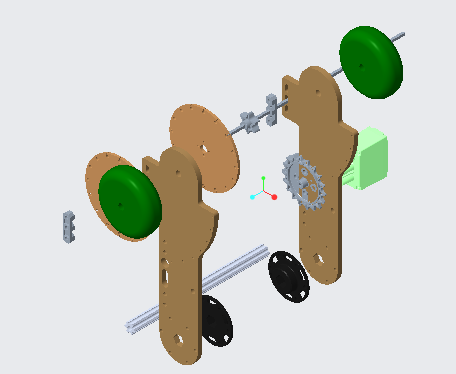
\includegraphics[width=0.8\textwidth]{Design_Overview/exploded_intake.PNG}
% \caption{Exploded View of the Intake Mechanism}
% \label{fig:exploded_intake}
% \end{figure}

% \begin{figure}[h!]
% \centering
% 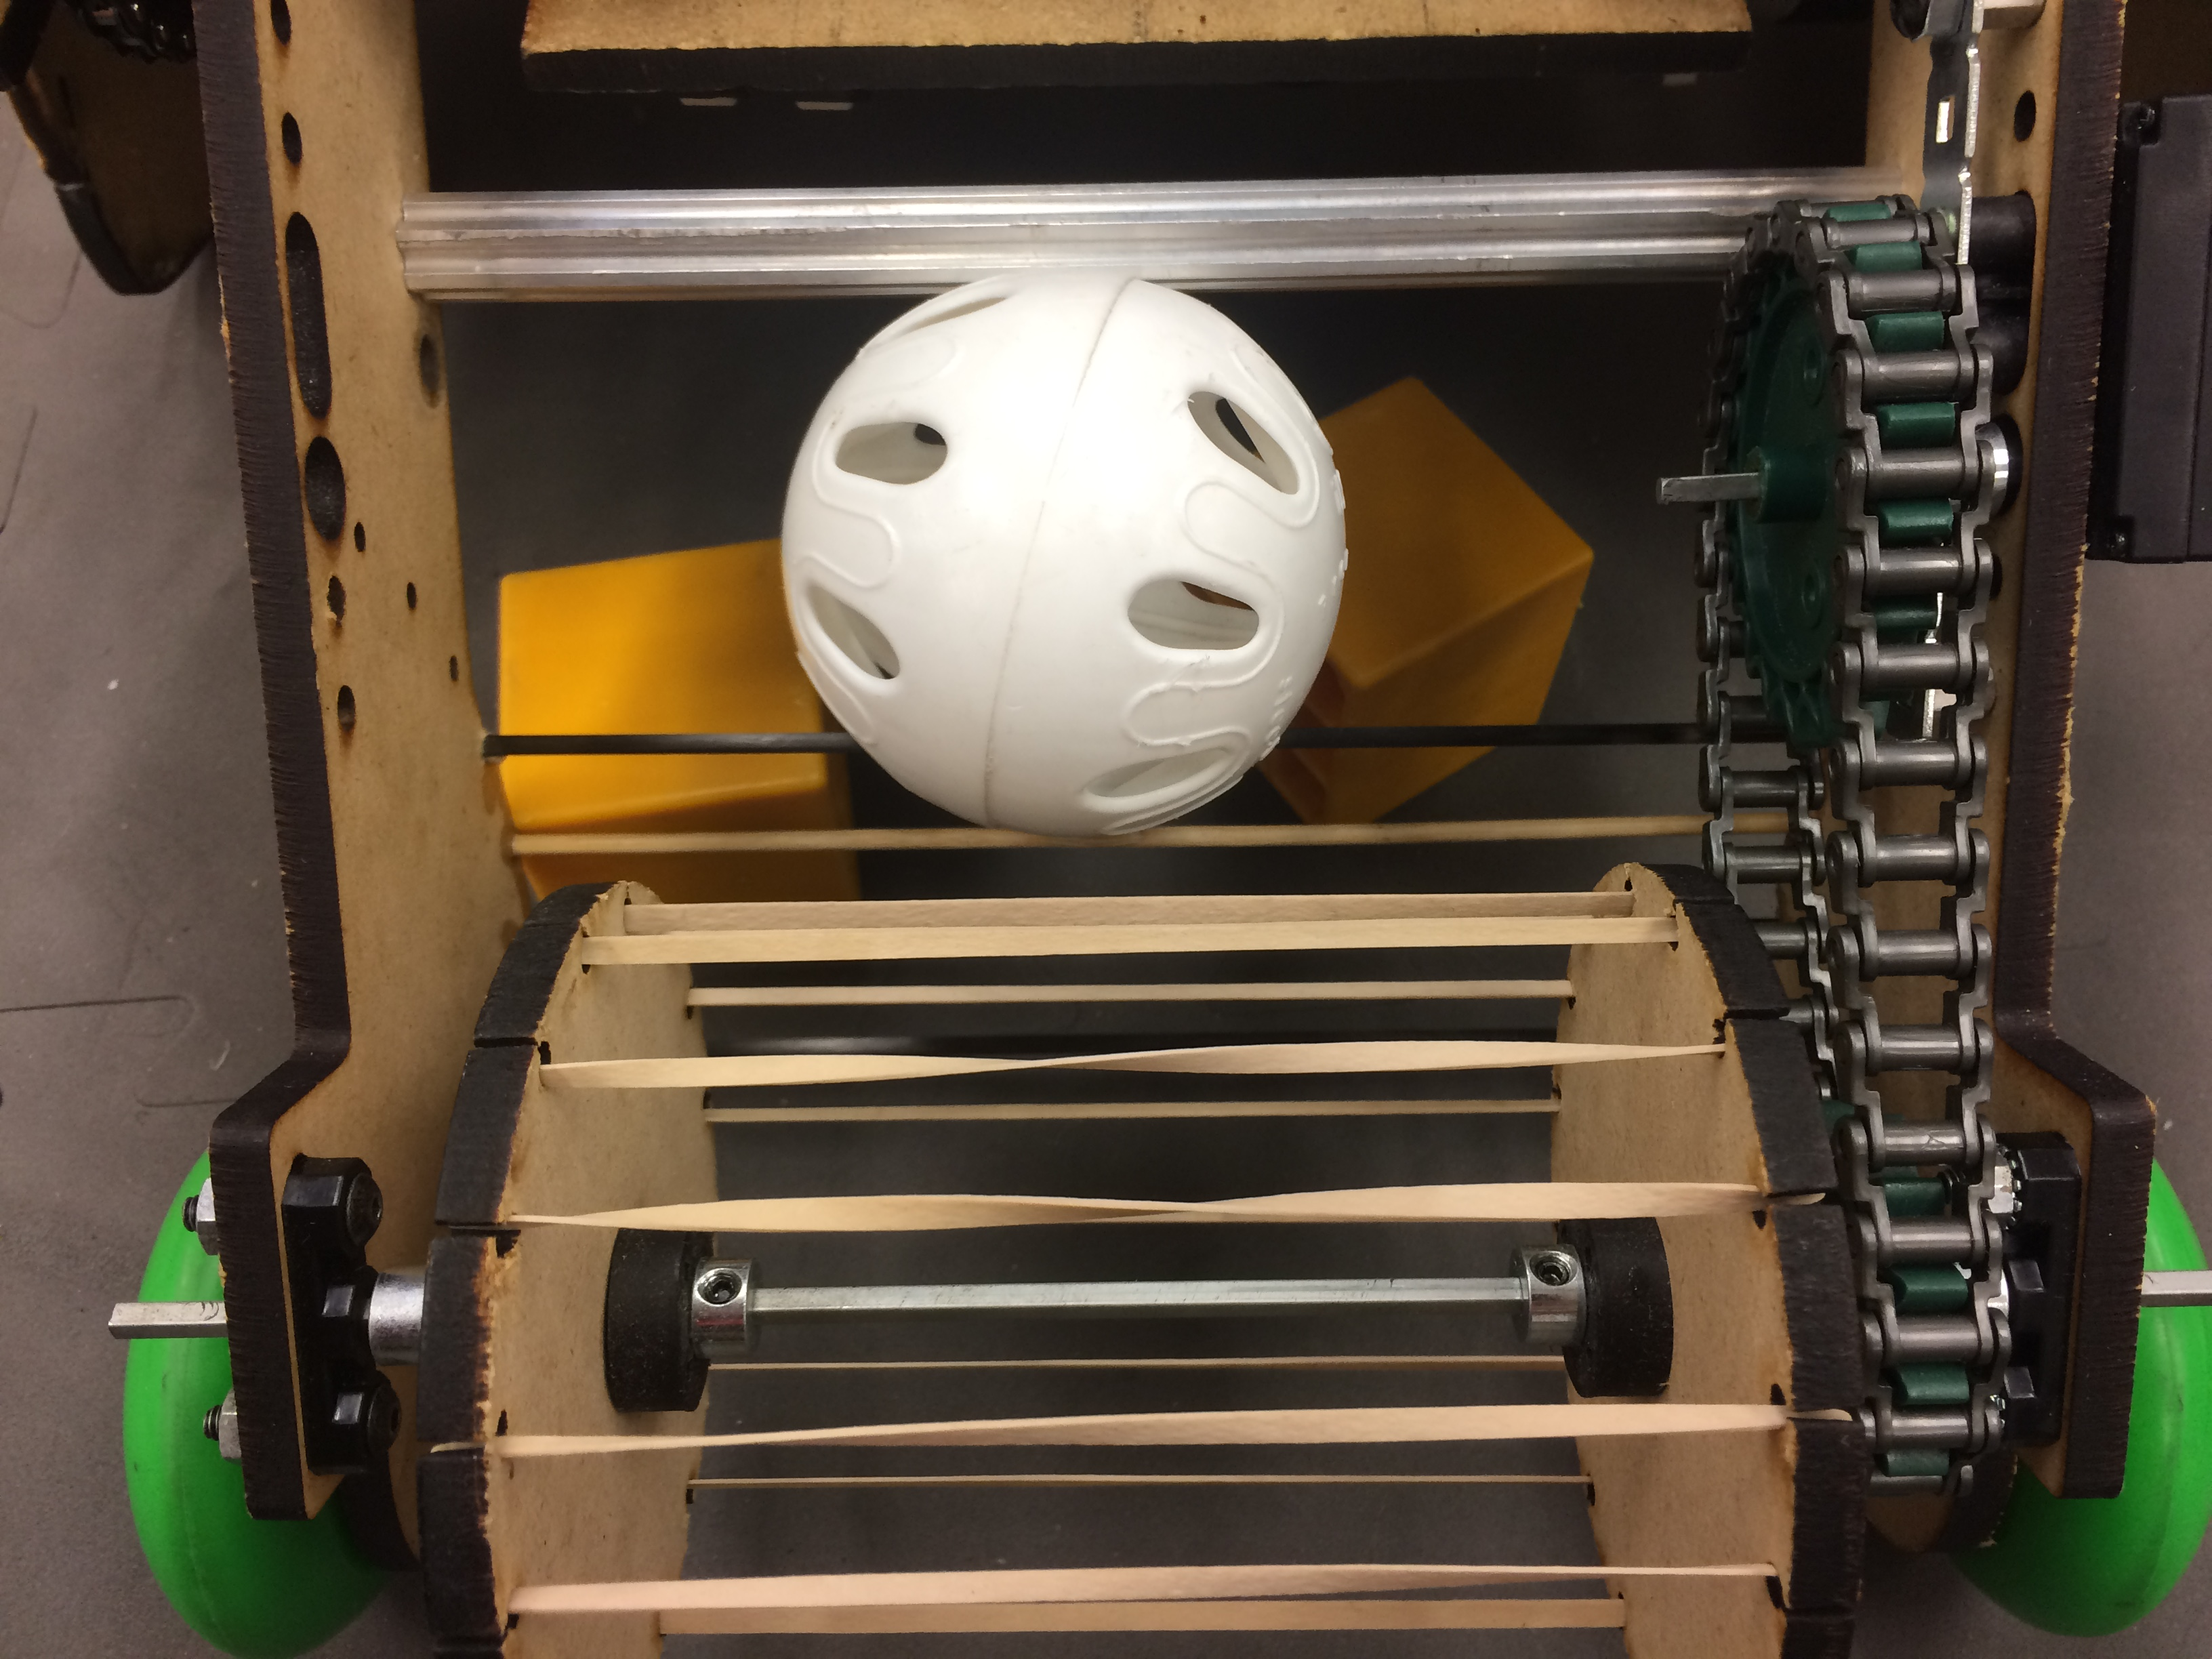
\includegraphics[width=0.8\textwidth]{Design_Overview/Sorting.JPG}
% \caption{Passive Sorting}
% \label{fig:sorting}
% \end{figure}

% \subsection*{Modelling \& Simulation}
% Much like all of our other mechanisms, we designed and simulated the intake using body and motion skeletons in PTC Creo. The most challenging issue with designing the intake was determining how far forward the rubberband wheels would be, as well as the size of the wheel itself. To make this easier on ourselves, we created sketches of the silver and gold minerals in the body skeleton and referenced it to design a smooth curve upwards that would maintain contact with the intake wheel. \hl{Our use of skeletons makes part implementation simple and fast, and facilitated continuous design iteration.} See below in Figures \ref{fig:skel_intake} and \ref{fig:skel_intake_use} to see how we implemented skeletons into our design. 

%    \begin{figure}[ht!]
% 	\centering
% 	\begin{minipage}{.48\textwidth}
% 	  \centering
% 	  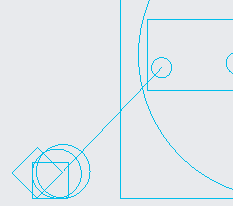
\includegraphics[width=0.8\linewidth]{Design_Overview/skel_intake.PNG}
% 	  \caption{The Intake Arm and Minerals in the Body Skeleton}
% 	  \label{fig:skel_intake}
% 	\end{minipage}%
% 	\begin{minipage}{.48\textwidth}
% 	  \centering
% 	  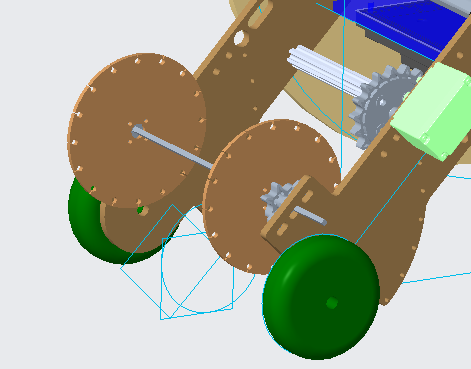
\includegraphics[width=0.8\linewidth]{Design_Overview/skel_intake_in_use.PNG}
% 	  \caption{The Skeleton in Use with Intake}
% 	  \label{fig:skel_intake_use}
% 	\end{minipage}
% 	\end{figure}

% \subsection*{The Phillip Mech}
% At the back of the intake, we have a mechanism to transfer the silver into the shooter (something our team refers to as Phillip). This consits of a REV servo that flips up. The arm is made of laser cut mdf made to have specially bent piano wire that works by having the intake bend the piano wire slightly out to get the silver in and then bends back to normal when the silver gets all the way in. The reason we use piano wire is that it holds its shape really well which means that it is hard to bend permanently but is easy to flex outward to allow for the silver to fall into the tray that goes up to the shooter.

%    \begin{figure}[ht!]
% 	\centering
% 	\begin{minipage}{.48\textwidth}
% 	  \centering
% 	  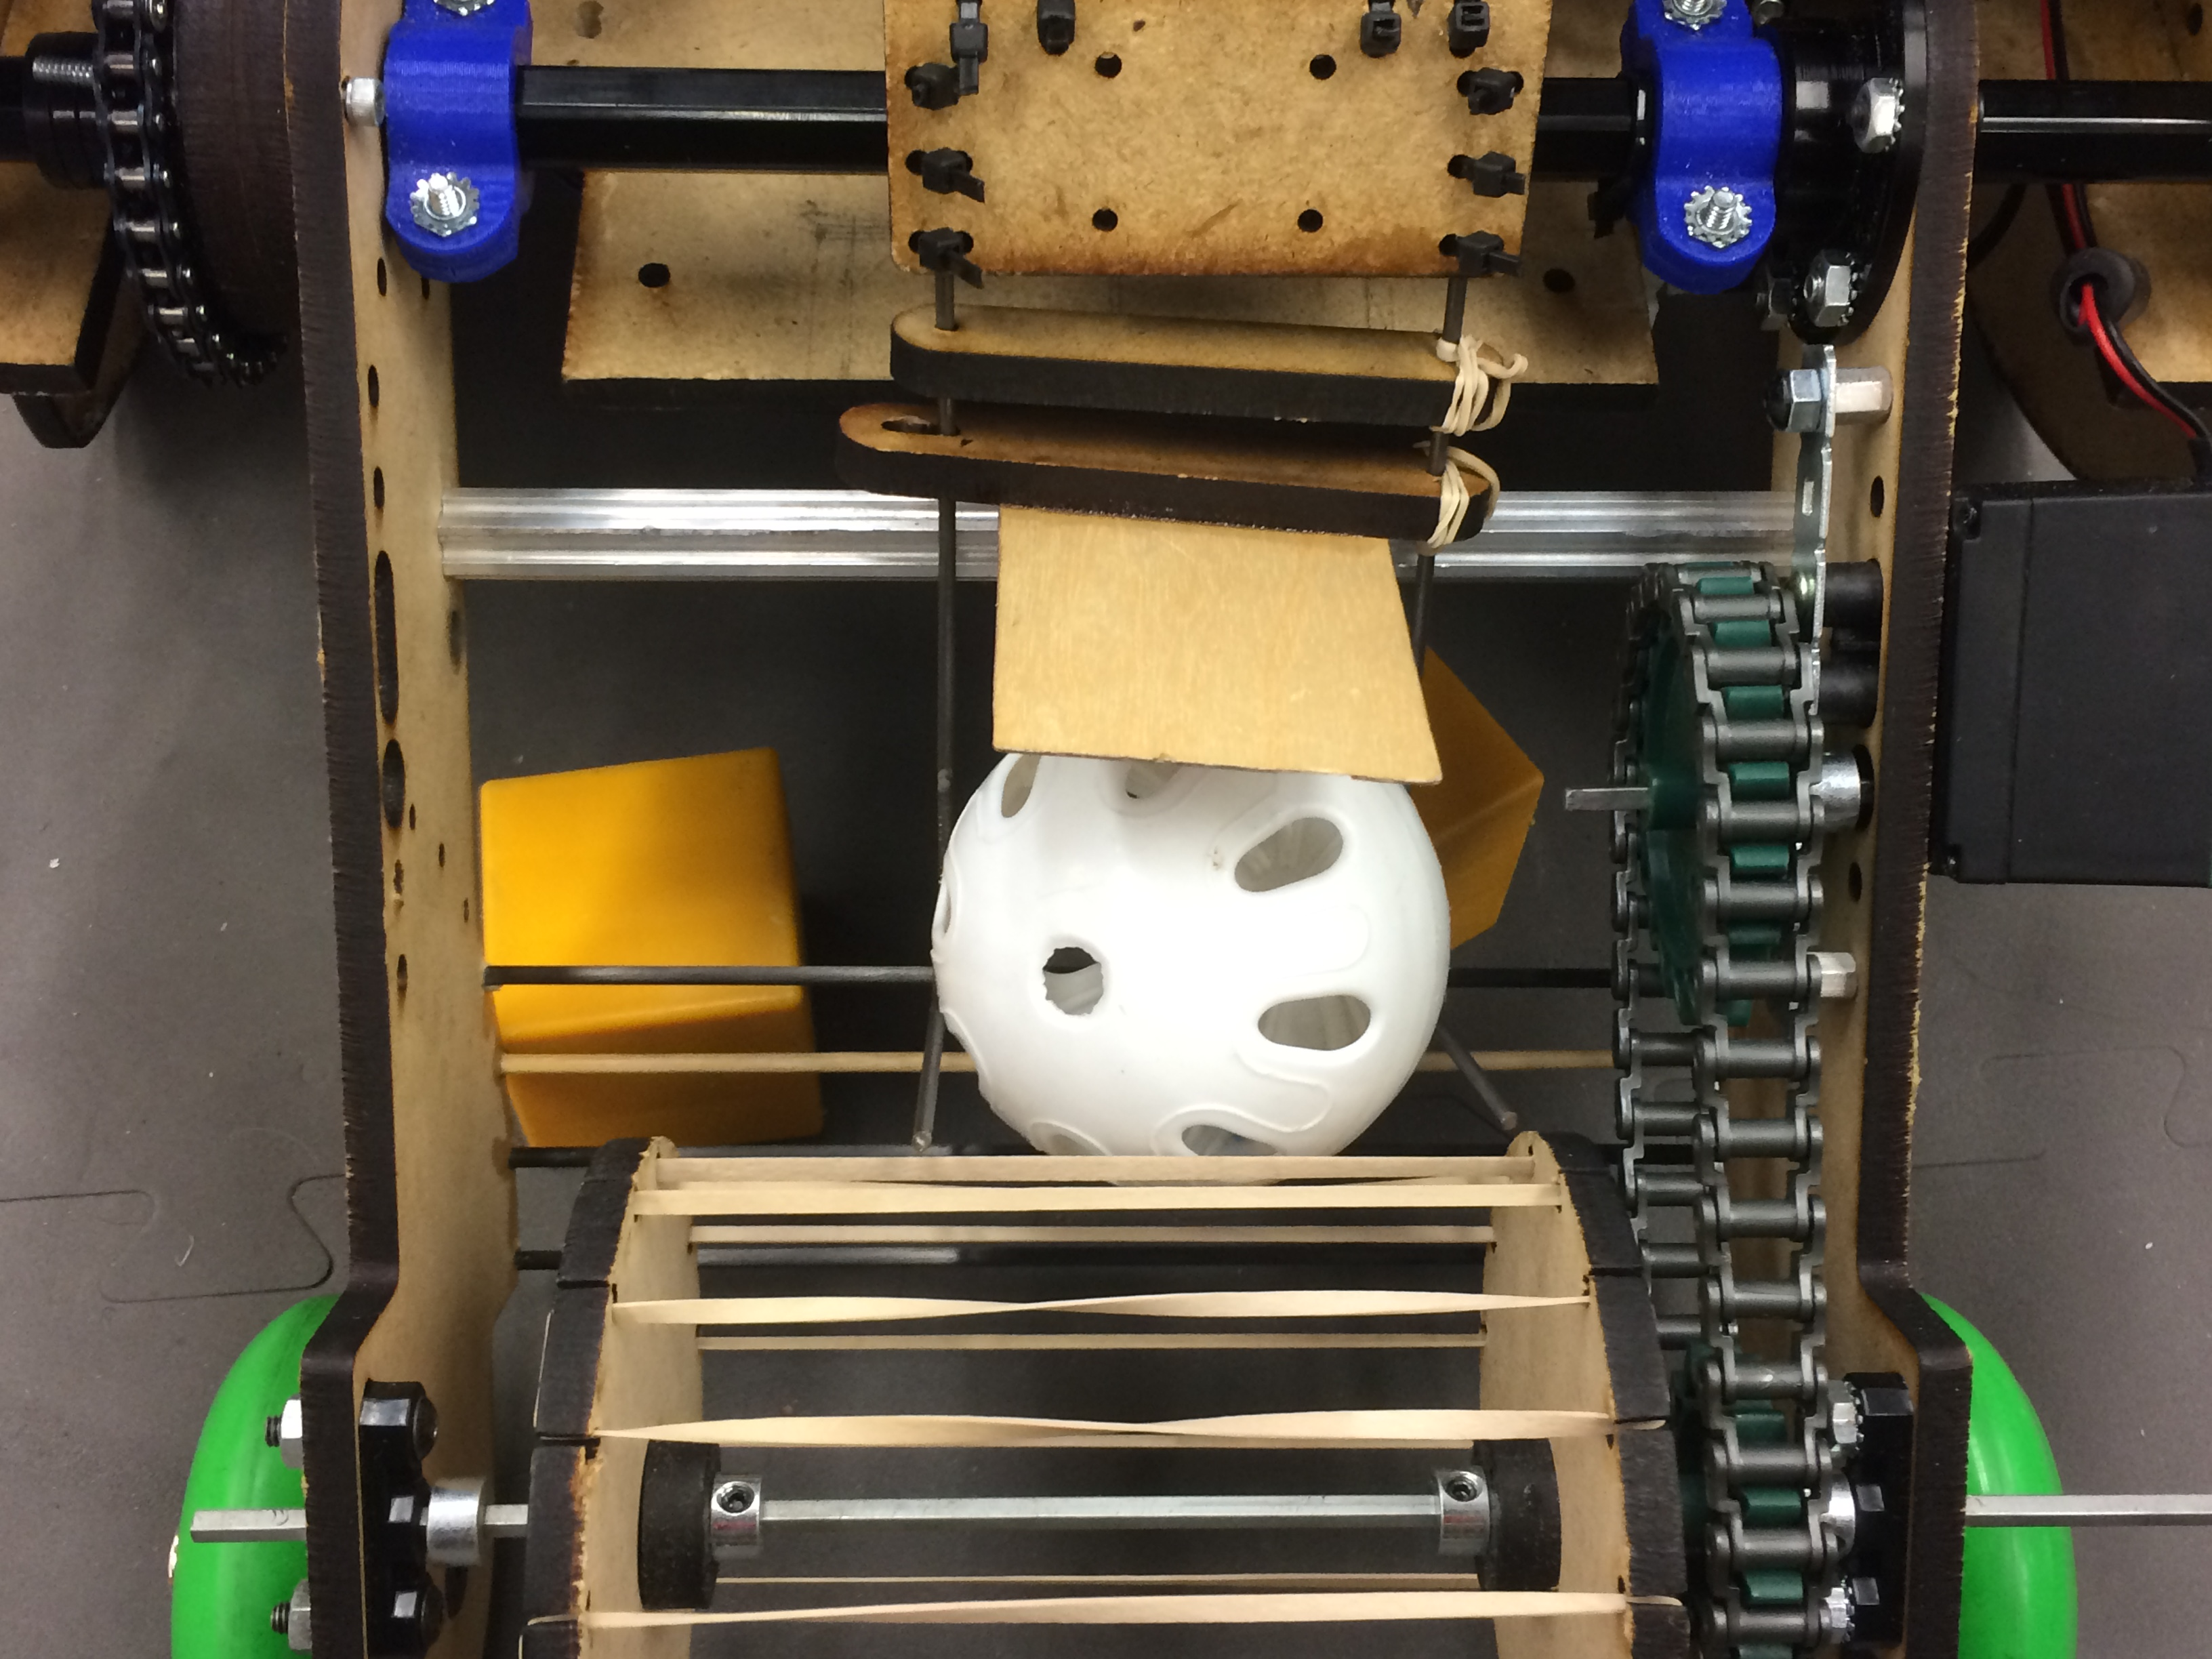
\includegraphics[width=0.8\linewidth]{Design_Overview/Phillip_1.JPG}
% 	  \caption{Loading The Transfer Mechanism}
% 	\end{minipage}%
% 	\begin{minipage}{.48\textwidth}
% 	  \centering
% 	  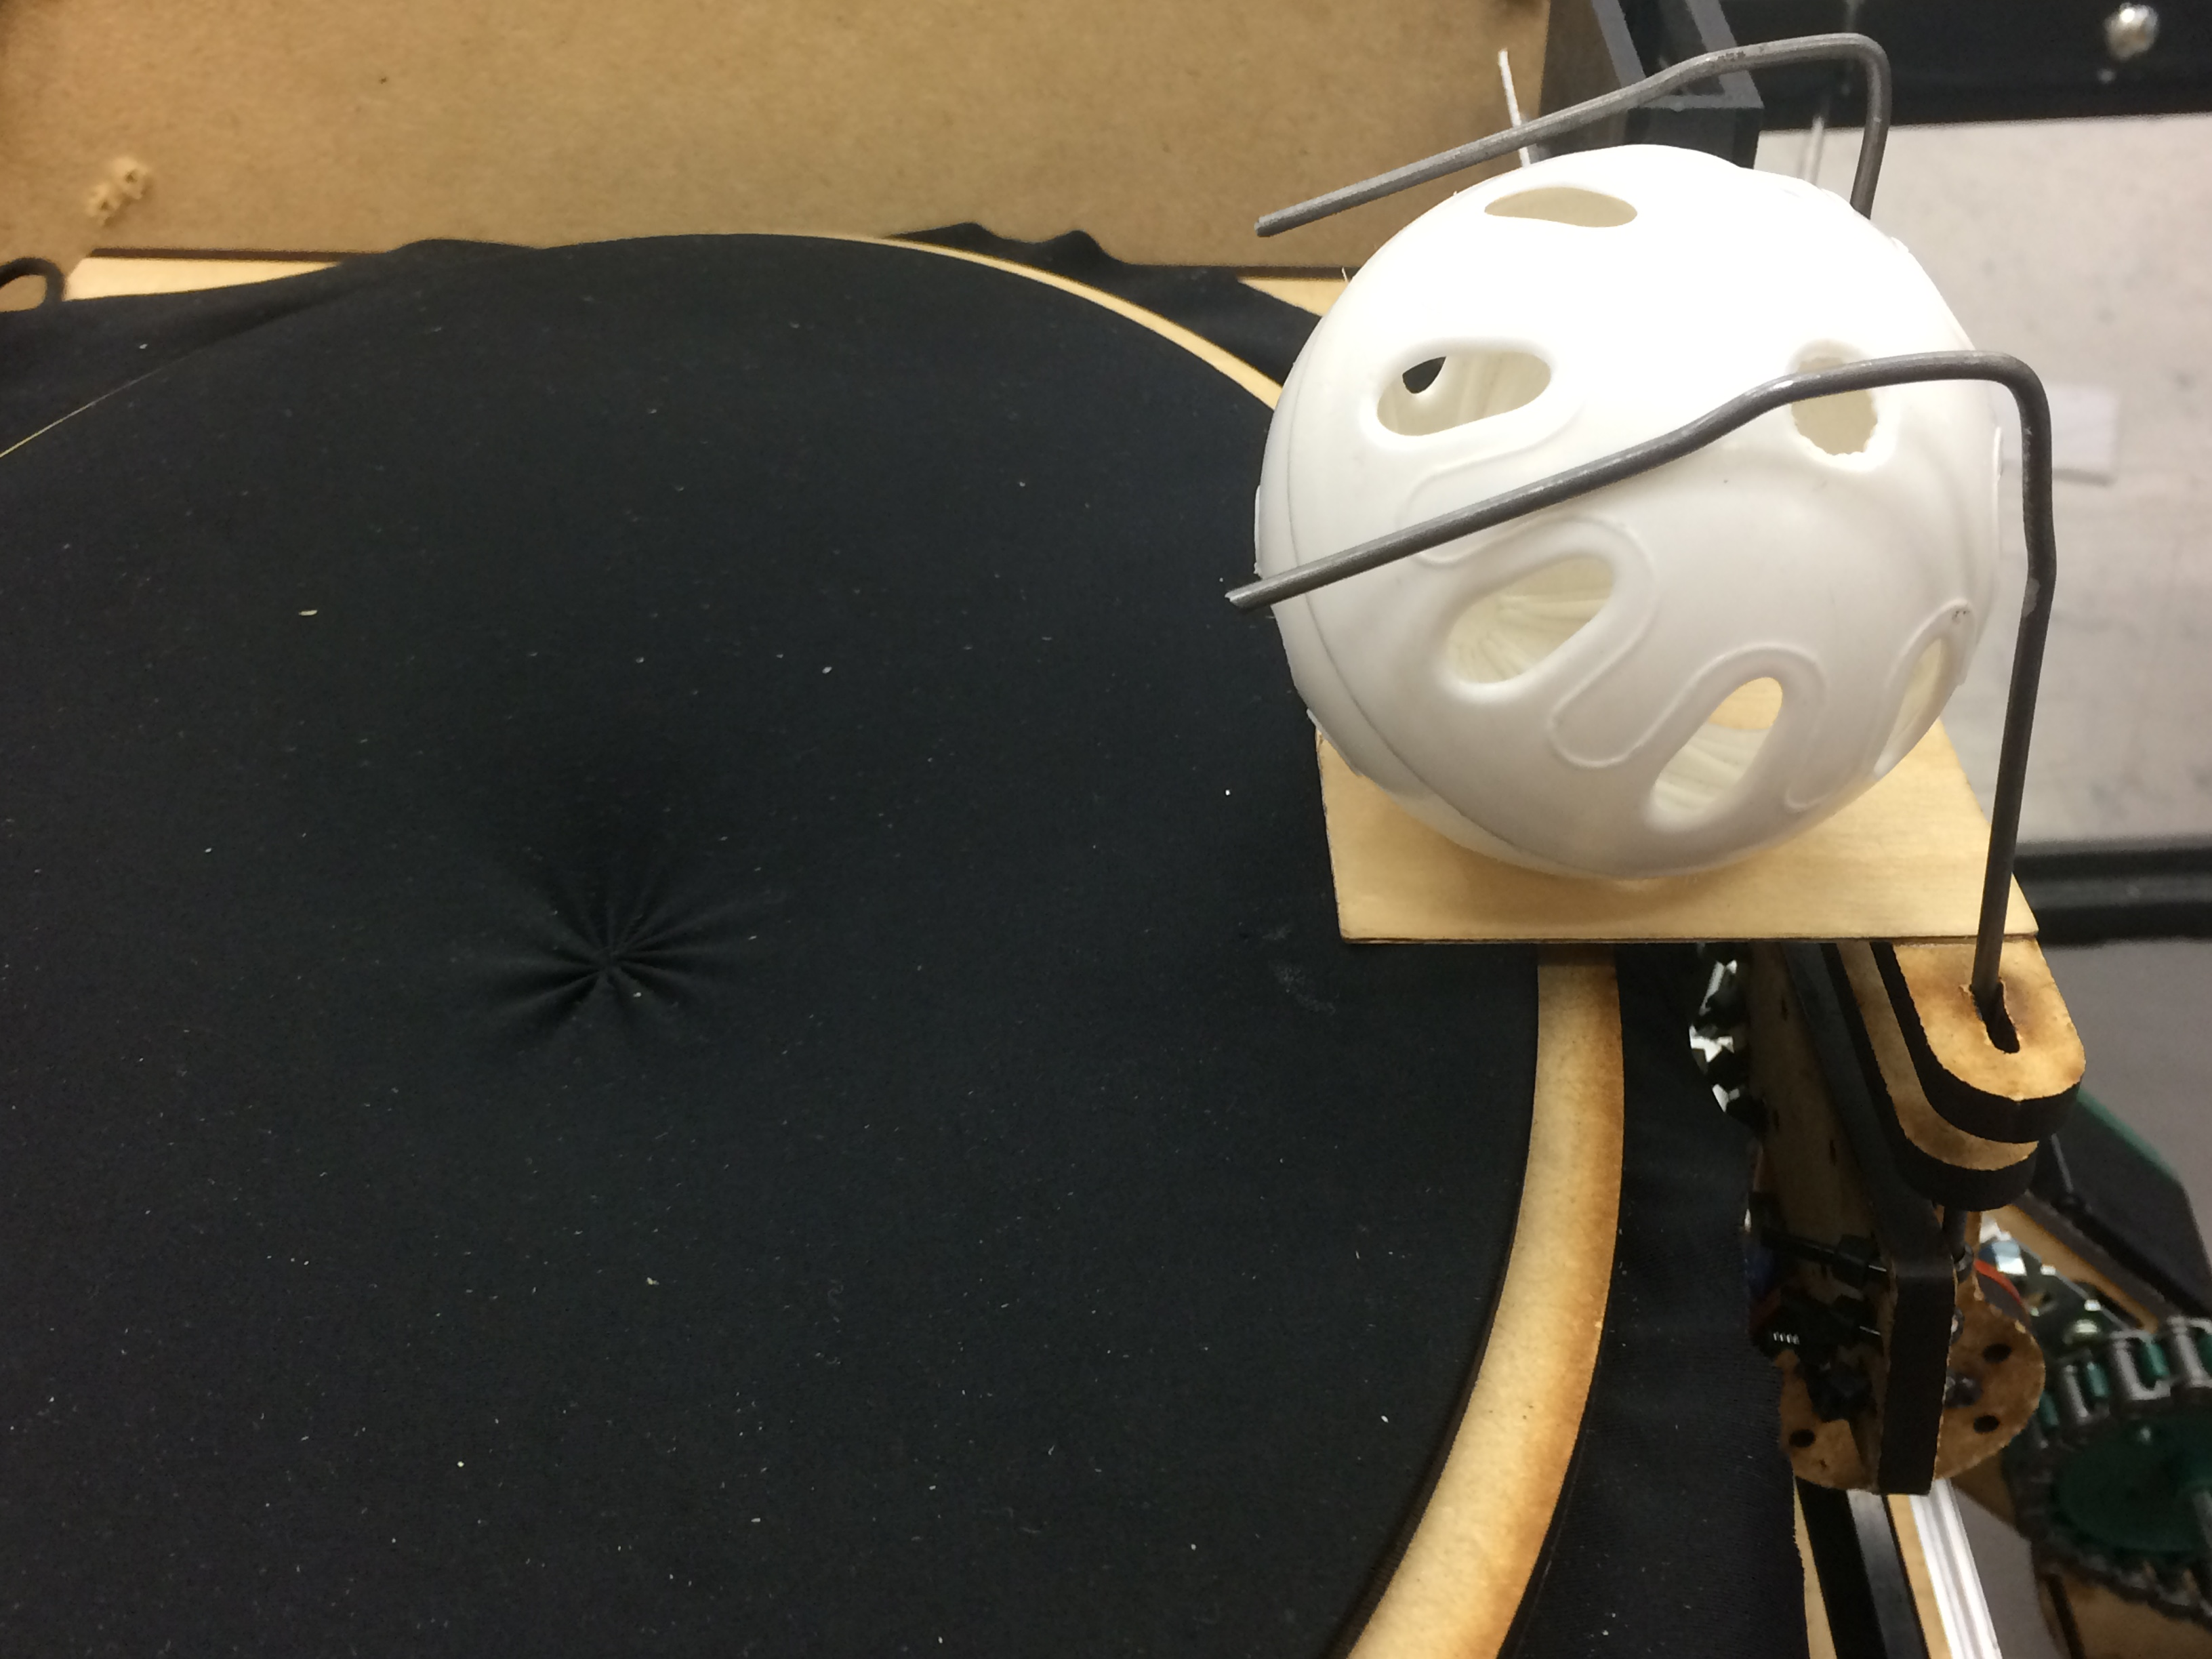
\includegraphics[width=0.8\linewidth]{Design_Overview/Phillip_2.JPG}
% 	  \caption{Transfer Mechanism Deposit to the Shooter}
% 	\end{minipage}
% 	\end{figure}

\subsection*{Iterations}
Initially, we built our intake to utilize a grabbing mechanism rather than a sweeper. Although our grabber became quite effective after making several tweaks to its design, we felt that we had hit a ceiling for its efficiency. Additionally, it is much harder to pick up freight in autonomous with a grabbing mechanism compared to with a spinner intake. Seeing this, we tested with a couple of types of spinners, including a roller wrapped in surgical tubing, and found the sweeper design to be most effective. 


% PUT THIS PHTOTO HERE: Design_Intake_Image3

One of the early designs of a spinner intake that we made had the sweeper positioned at a fixed height. We quickly found that this limited us to only being able to reliable hold the blocks which are smaller than the wiffle balls. When we tried to increase the height of the sweeper to allow us to intake the balls, we found that the blocks would slip out of the intake as we pivoted the arm, sometimes launching the block and incurring penalties. Observing this, we created our pivoting sweeper which can much more effectively grab and hold freight of different sizes.

% PUT THIS PHTOTO HERE: Design_Intake_Image4

Another thing we learned from a previous spinner intake design was the effectiveness of different materials on the sweeper. We initially started testing with surgical tubing, a popular material for FTC intakes but found that it didn’t live up to the utility we had expected seeing so many teams use a similar design. Instead, we tried several different materials and designs that we came up with ourselves and found many of them to be much more successful than the surgical tubing. Ranging from zip ties to different types of foam, we tested many materials and forms, eventually finding rubber strips we had cut from a sheet of rubber to be most effective. To increase the effectiveness of the rubber flaps, we laser cut them to get a cleaner and more precise shape.


% \interesting{Iterative Design with the Intake}{design:6}

% \begin{figure}[htp]
% \centering
% 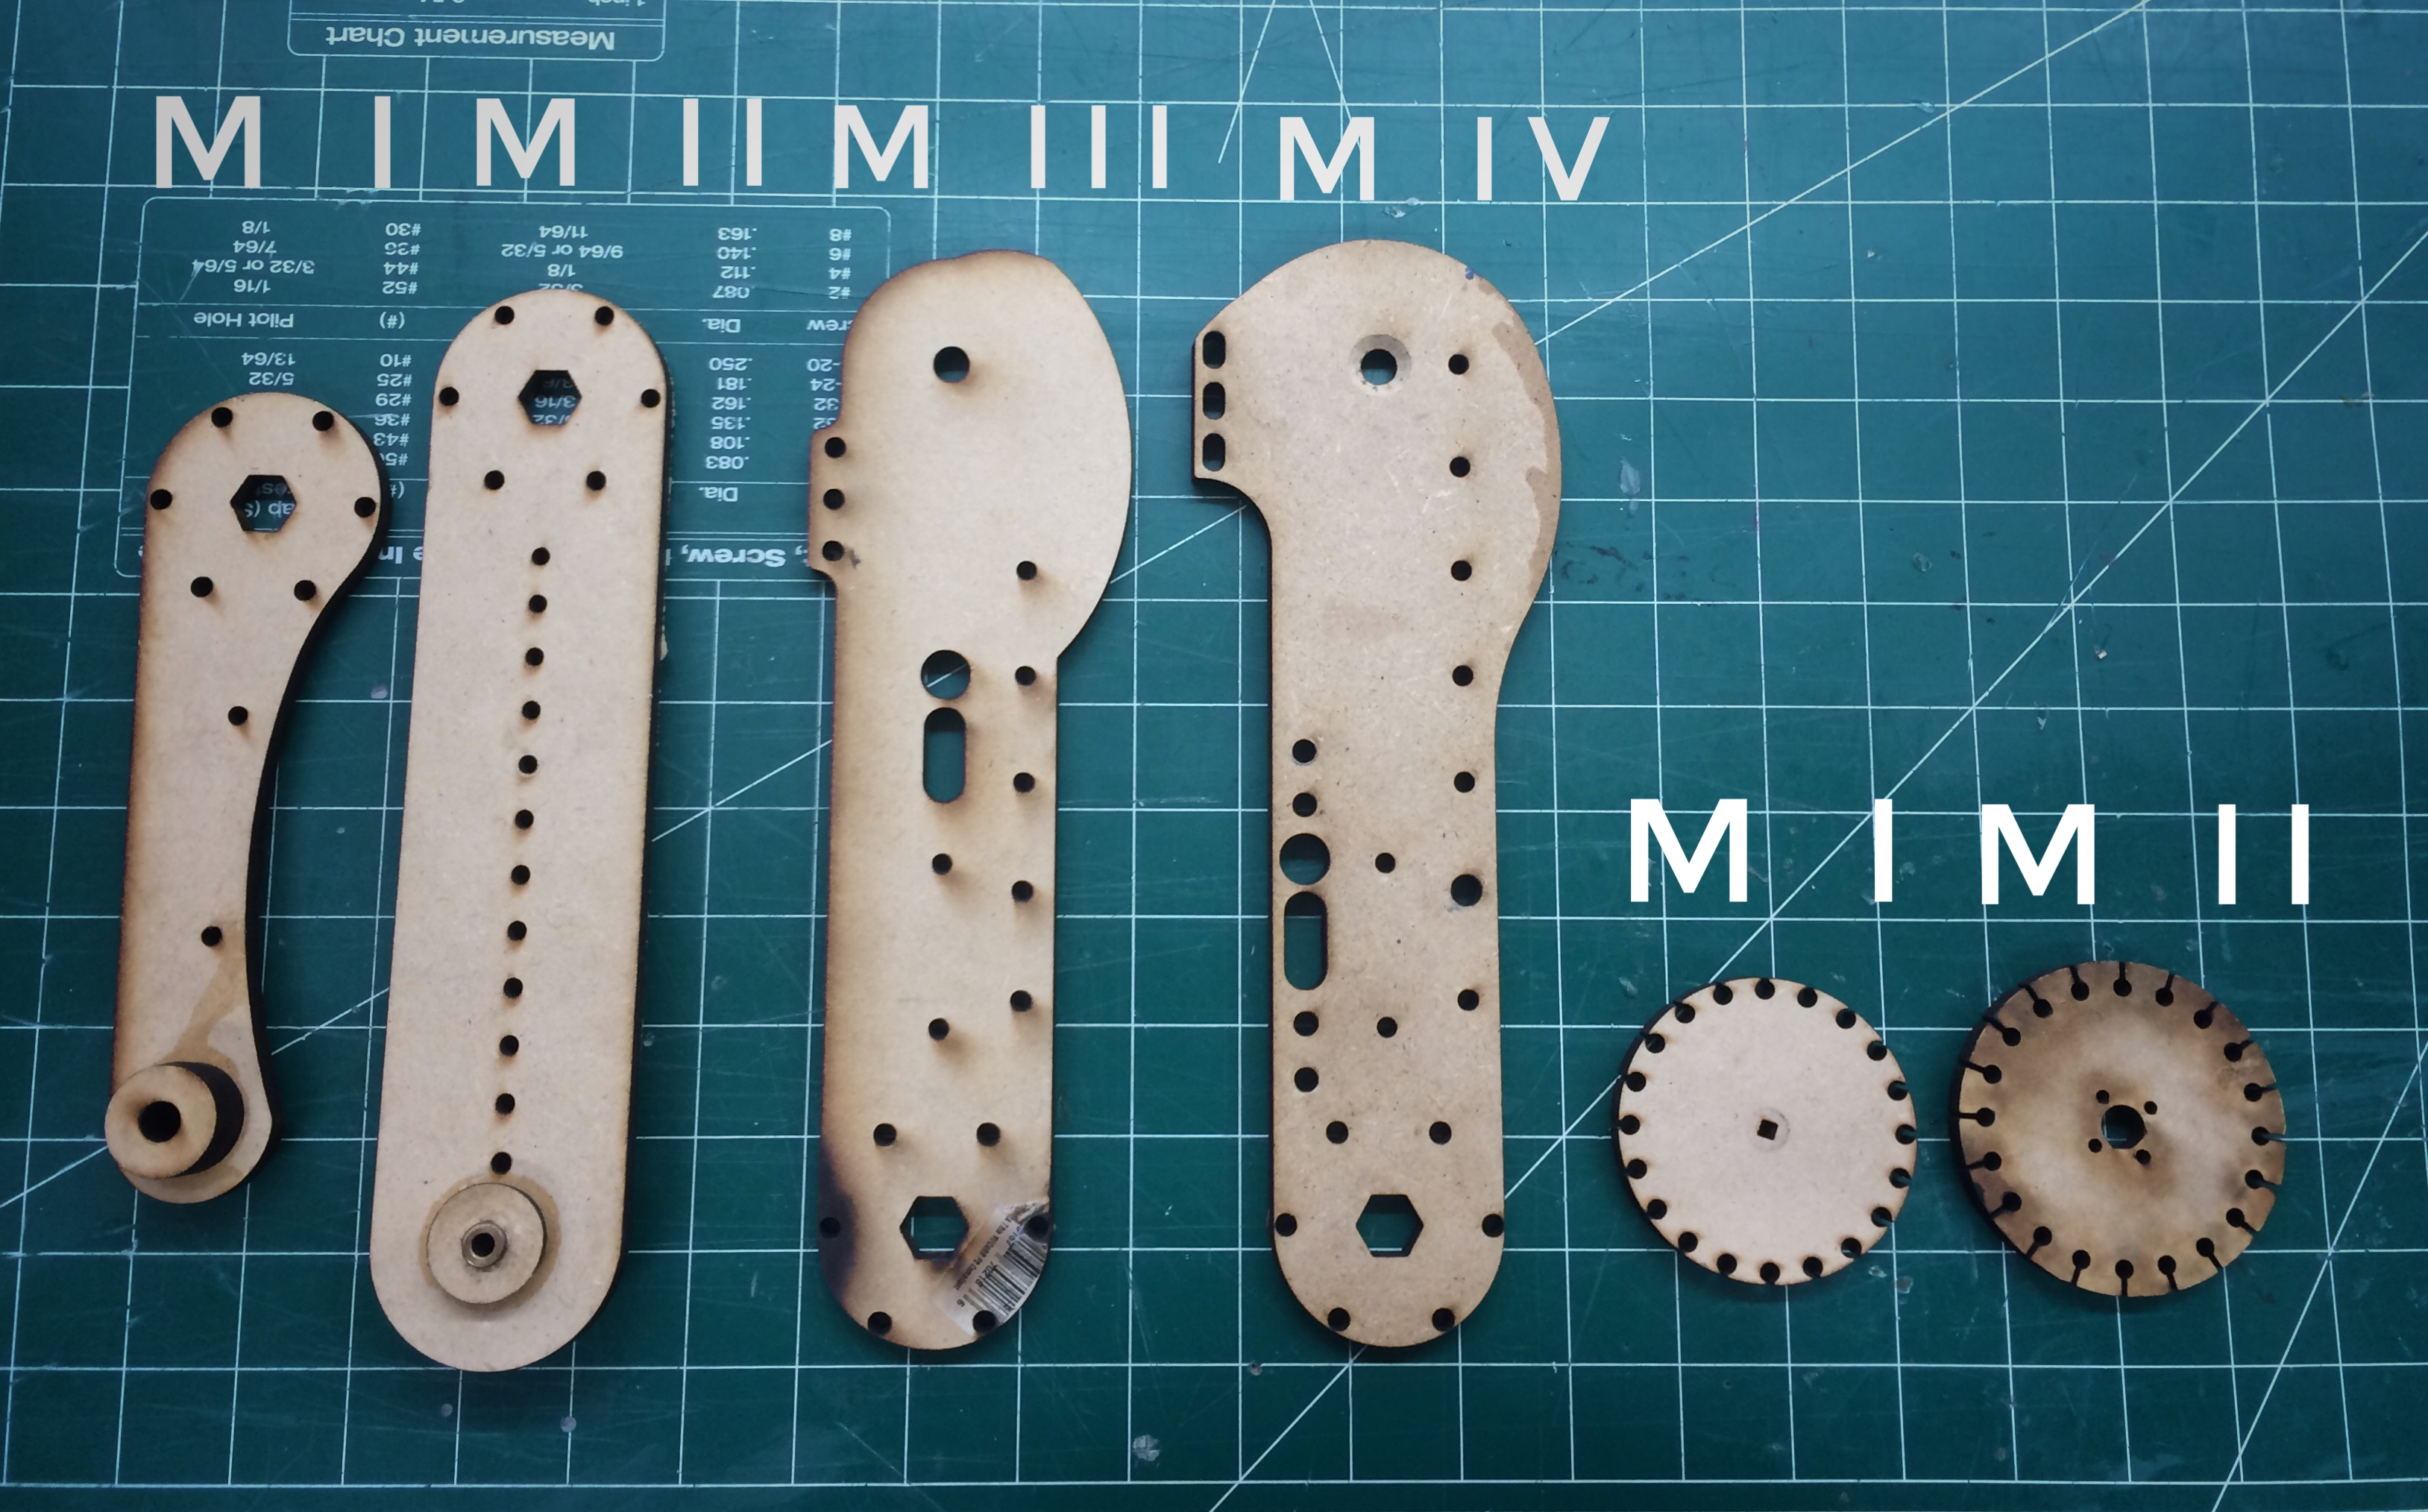
\includegraphics[width=.8\linewidth]{Design_Overview/Intake_Iteration.jpg}
% \caption{Design Iteration of the Intake, Mark I to IV}
% \label{fig:intake_it}
% \end{figure}

% \begin{figure}[htp]
% \centering
% \begin{minipage}{.32\textwidth}
%   \centering
%   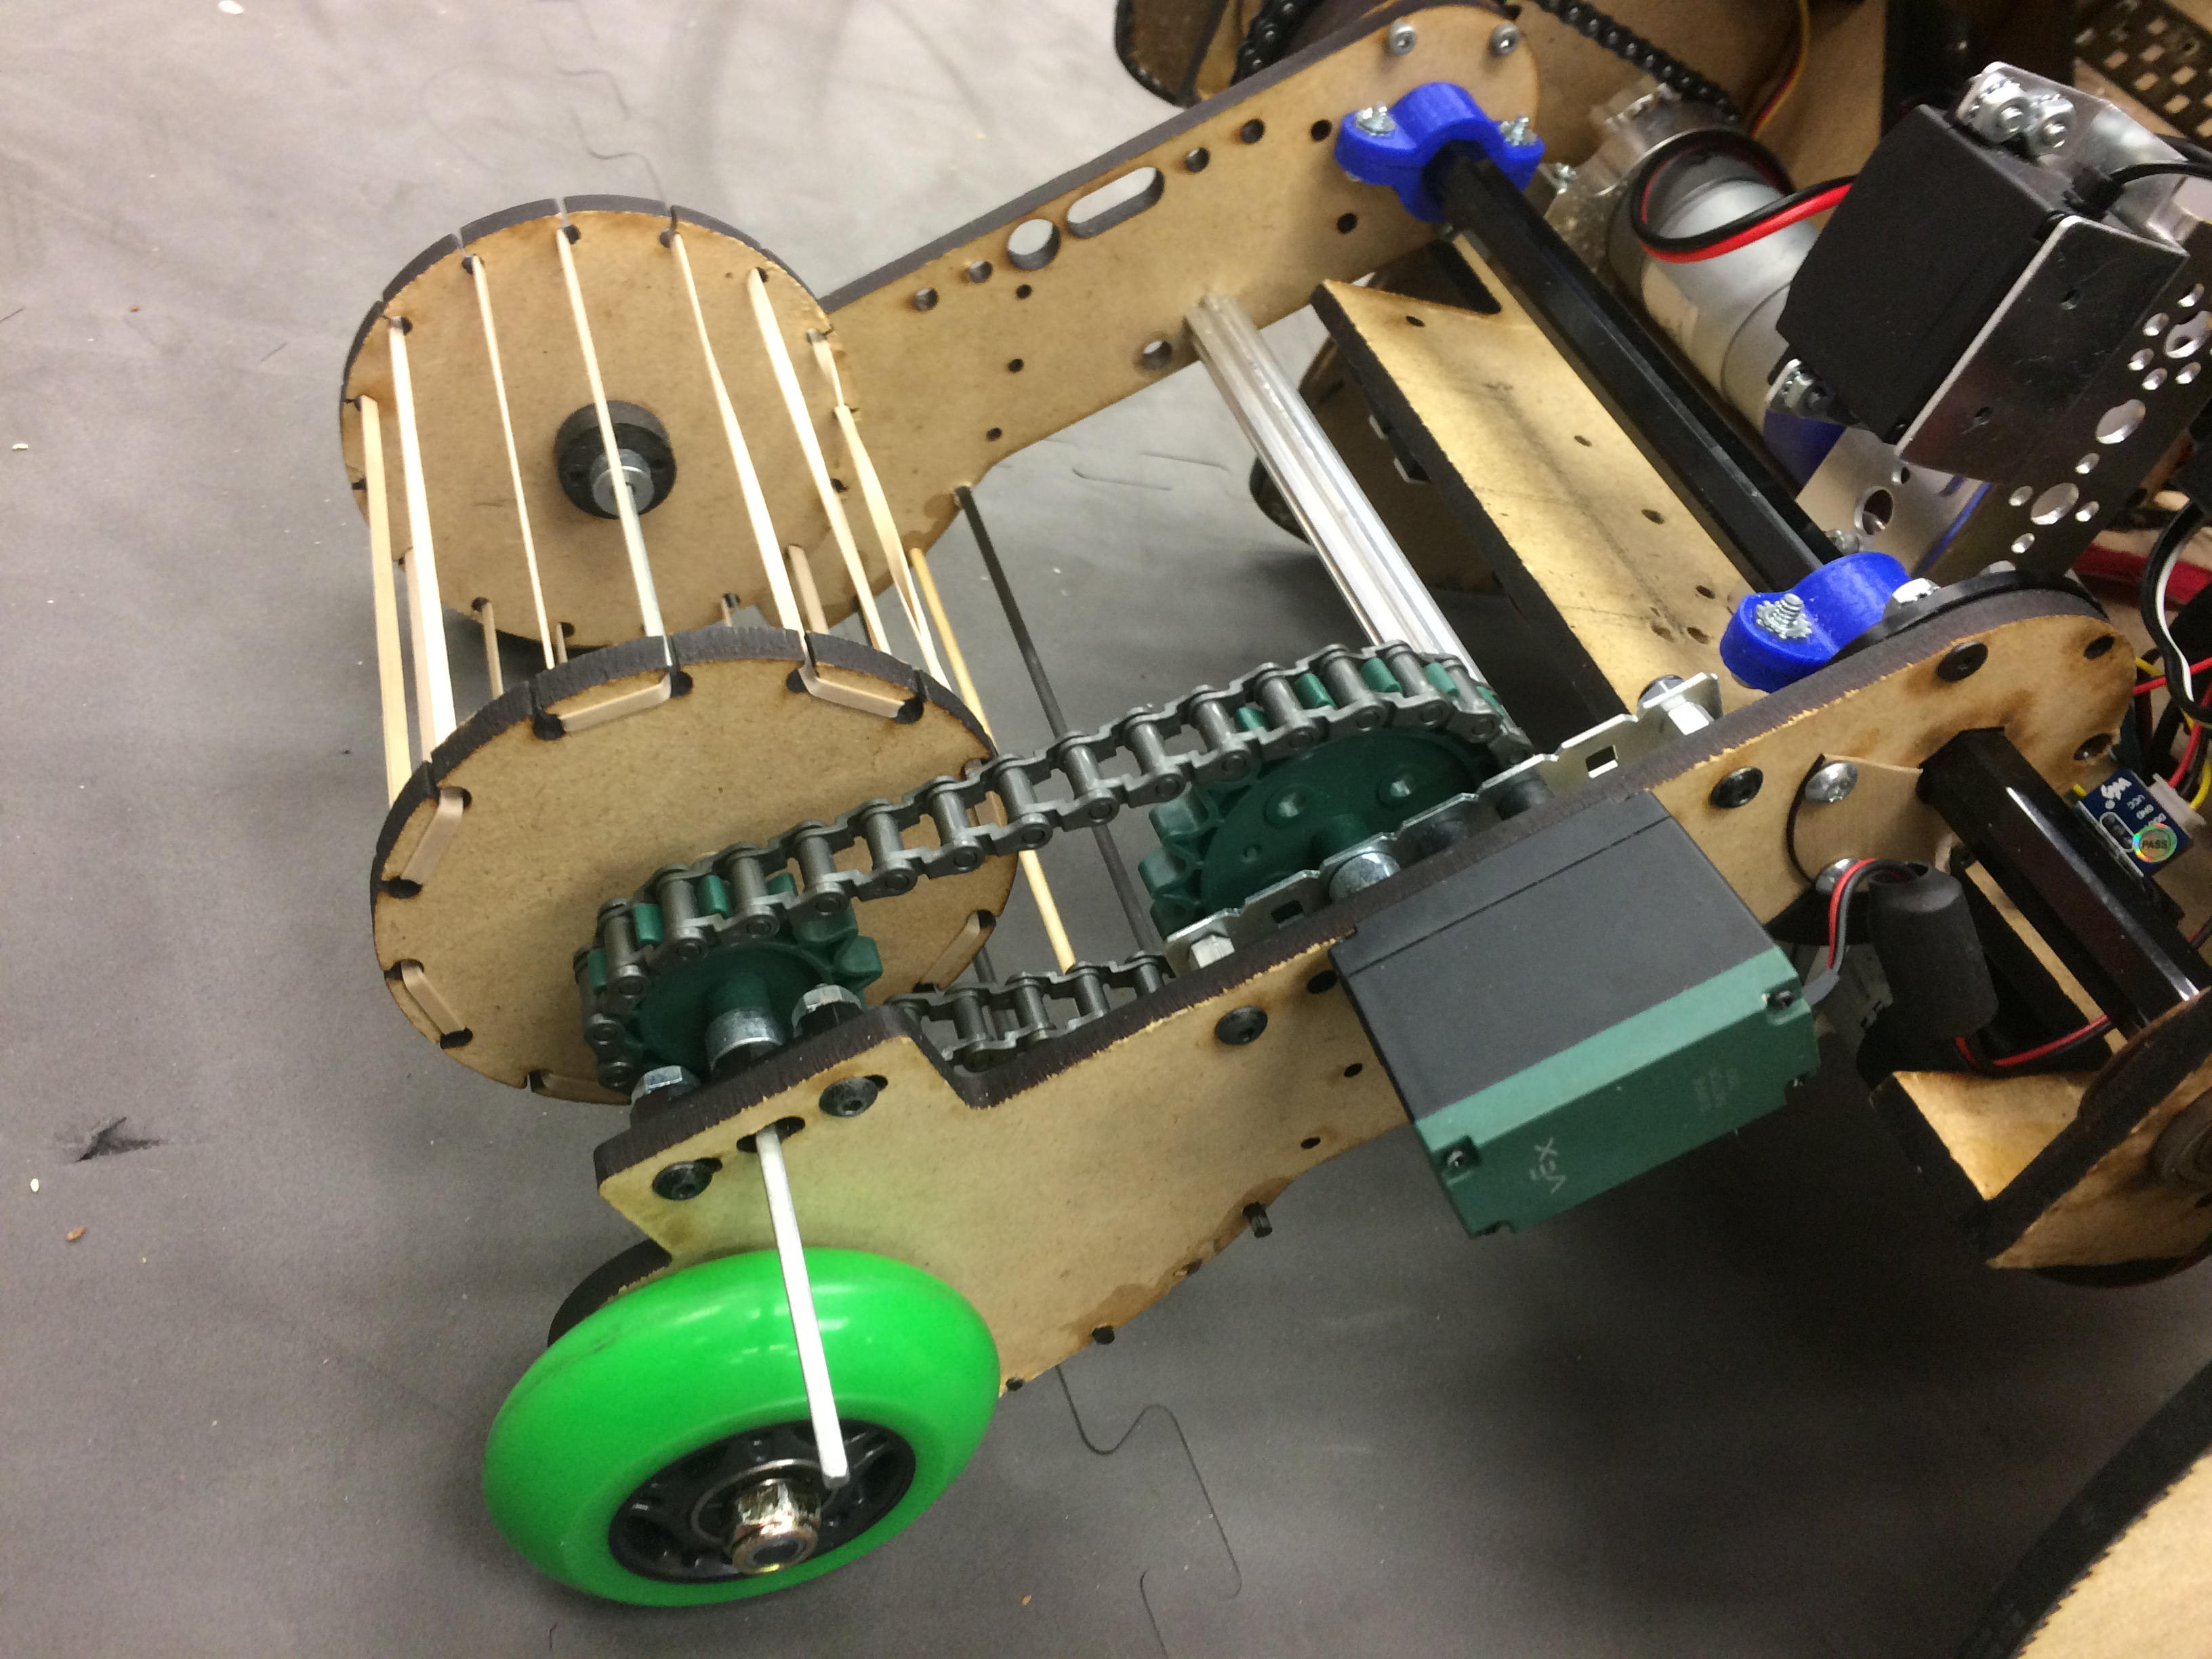
\includegraphics[width= .9\linewidth]{Design_Overview/Intake_Left.JPG}
% \end{minipage}%
% \hfill
% \begin{minipage}{.32\textwidth}
%   \centering
%   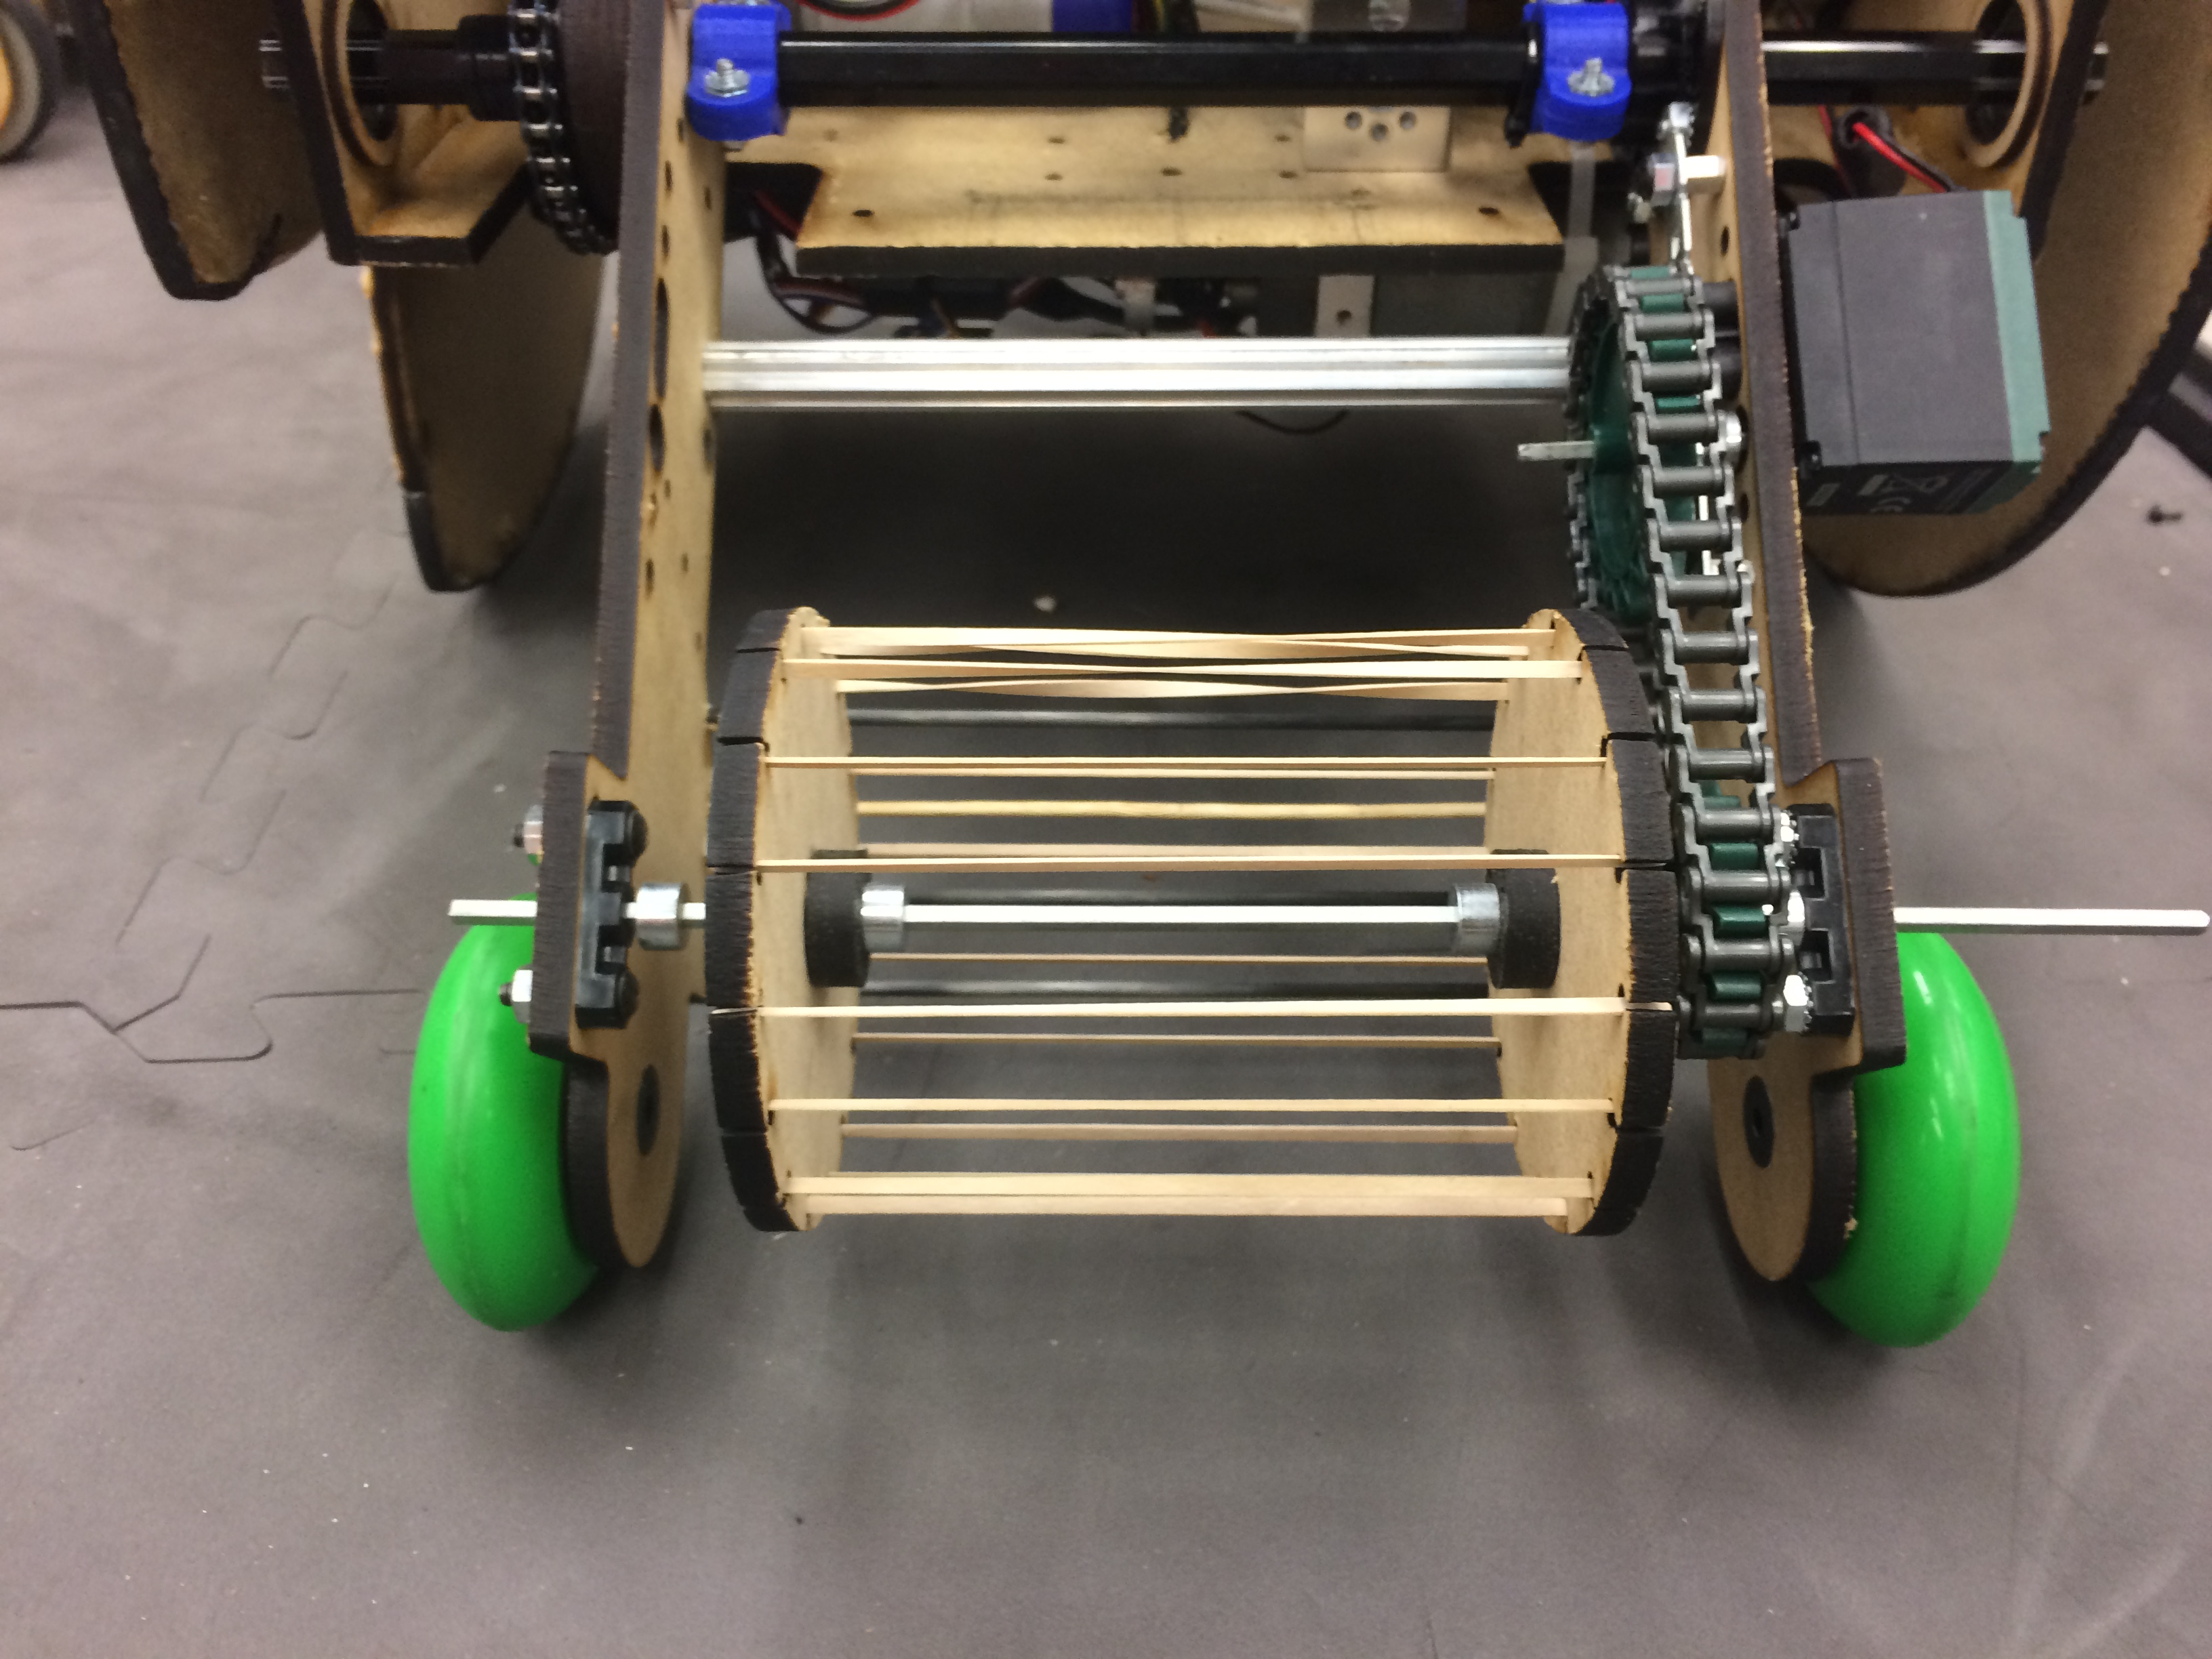
\includegraphics[width= .9\linewidth]{Design_Overview/Intake_Front.JPG}
% 	\caption{Final Intake, Mark V}
% 	\label{fig:triple_intake_IMG}
% \end{minipage}%
% 	\hfill
% \begin{minipage}{.32\textwidth}
%   \centering
%   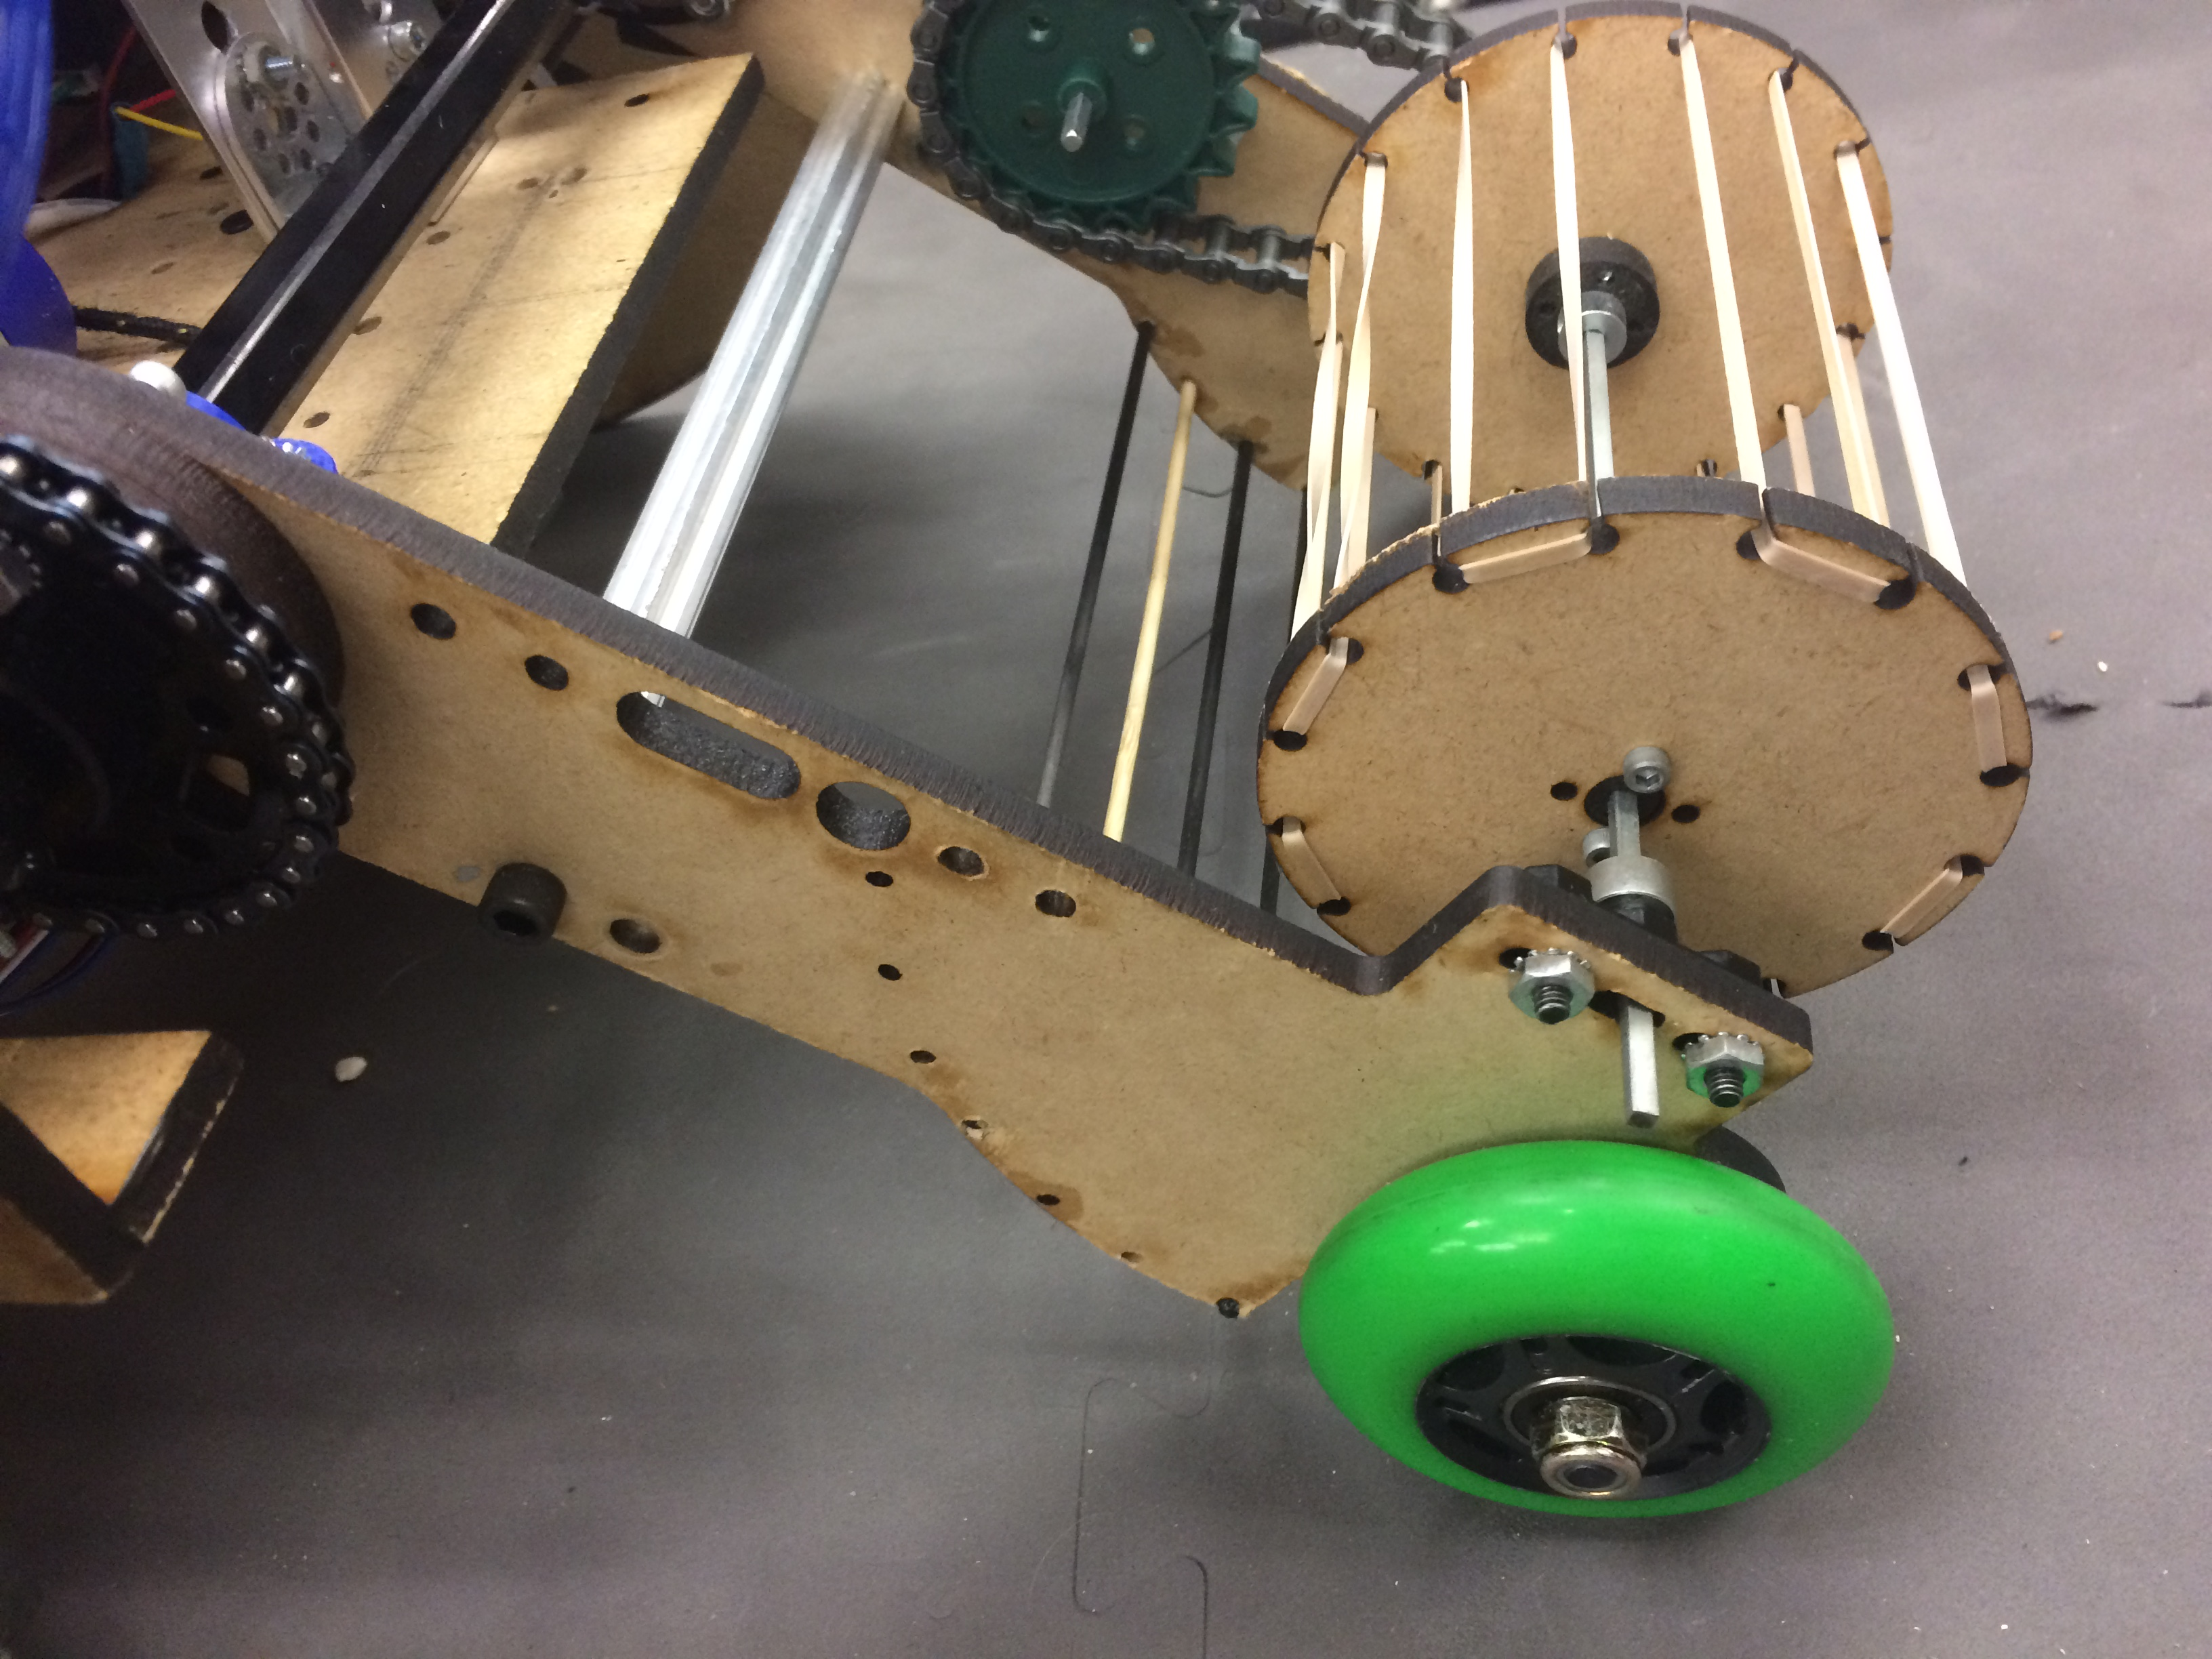
\includegraphics[width= .9\linewidth]{Design_Overview/Intake_Right.JPG}
% \end{minipage}
% \end{figure}

\subsection*{Sensors and Control}
We have one color sensor attached to the top of our intake to allow us to sense if we have grabbed a block during the autonomous period. This allows the robot to know when it should leave the warehouse to score the freight it has collected. It is also used to automatically raise the arm so we can get rid of any extraneous freight. 

\subsection*{Mechanism Accomplishments}
\begin{itemize}
    \item Allow for autonomous pick up
    \item Lightweight to reduce motor stress
    \item Firm block grip 
    \item Adapts to any size freight
\end{itemize} 